\section{稳健性检验}
\label{sec:robust}

本节按时间稳定性、制度设定、推断方法与样本宽度四类威胁检验前述结论，
并对照既有零结果。

\begin{table}[htbp]
\centering
\caption{子样本稳定性}
\label{tab:subsample}
\begin{threeparttable}
\small
\begin{tabular}{llrrr}
\toprule
时段 & 年份 & 门控夏普 & 等权夏普 & 夏普差值 \\
\midrule
前半段 & 2014--2019 & 0.549 & 0.369 & $+0.180$ \\
后半段 & 2020--2025 & 0.797 & 0.747 & $+0.049$ \\
\bottomrule
\end{tabular}
\begin{tablenotes}[flushleft]\footnotesize
\item 注：数值由主实验的年度窗口直接汇总（与表 \ref{tab:main} 同源）。段内先对随机种子取平均，再对年份取平均。
\end{tablenotes}
\end{threeparttable}
\end{table}

表 \ref{tab:subsample} 显示门控优势的时间衰减：相对等权的夏普差值在前半段
（2014--2019）为 $+0.180$，在后半段（2020--2025）降至 $+0.049$。
两段内门控的绝对表现都上升（0.549 $\to$ 0.797），等权基准上升更多
（0.369 $\to$ 0.747），相对优势因此收窄。两个机制可以解释这一模式：
2014--2019 年 A 股经历若干次幅度较大的制度切换（2015 年杠杆牛市与随后的调整、
2016 年熔断），状态识别的价值较高；2020 年后风格切换更频繁但幅度更温和，
且股票池由 428 只扩大至 523 只，等权基准的分散化程度提高。
无论何种解释，基于全样本平均的门控优势结论都需要补充子样本稳定性。

\begin{table}[htbp]
\centering
\caption{制度定义与制度数的稳健性}
\label{tab:statedef}
\begin{threeparttable}
\small
\begin{tabular}{llrr}
\toprule
制度变量 & 制度数 & 平均夏普 & 相对等权夏普差值 \\
\midrule
12 个月市场收益 & 2 & 0.631 & $+0.073$ \\
12 个月市场收益 & 3 & 0.722 & $+0.164$ \\
6 个月市场波动 & 2 & 0.668 & $+0.110$ \\
6 个月市场波动 & 3 & 0.618 & $+0.060$ \\
1 年市场回撤 & 2 & 0.702 & $+0.144$ \\
1 年市场回撤 & 3 & 0.561 & $+0.003$ \\
横截面离散度 & 2 & 0.705 & $+0.147$ \\
横截面离散度 & 3 & 0.619 & $+0.060$ \\
\bottomrule
\end{tabular}
\begin{tablenotes}[flushleft]\footnotesize
\item 注：制度以 one-hot 形式并入门控输入，其余设定不变。
数值为 12 个测试年份的平均（单一种子）。差值为相对同期等权基准的夏普差。
\end{tablenotes}
\end{threeparttable}
\end{table}

表 \ref{tab:statedef} 显示结果对制度定义敏感。夏普表现区间为 0.561（1 年回撤，$S=3$）
至 0.722（12 个月收益，$S=3$），跨度约 0.16，与门控相对等权的整体优势（$+0.12$）
同量级，制度变量的选择本身贡献了与机制同量级的不确定性。
「12 个月市场收益 + 3 状态」在 $S=2$ 与 $S=3$ 下表现均较好，
其余三种定义下 $S=2$ 优于 $S=3$，说明在这些定义下增加制度数带来的估计误差成本
超过互补性收益。相对优势在八种设定下全部为正（$+0.003$ 至 $+0.164$），
收益方向不依赖特定定义，量级则高度依赖定义。

\begin{table}[htbp]
\centering
\caption{自助区块长度对阈值检验的影响}
\label{tab:block}
\begin{threeparttable}
\small
\begin{tabular}{lrrr}
\toprule
区块长度（月） & 一阶 $p$ 值 & 二阶 $p$ 值 & 5\% 水平是否显著 \\
\midrule
3 & 0.055 & 0.018 & 仅二阶 \\
6 & 0.048 & 0.030 & 一阶与二阶 \\
12 & 0.060 & 0.065 & 均不显著 \\
24 & 0.060 & 0.095 & 均不显著 \\
\bottomrule
\end{tabular}
\begin{tablenotes}[flushleft]\footnotesize
\item 注：$p$ 值为自助分布中不小于观测统计量的比例。区块越长，
保留的序列相关越多，噪声底线越高，检验越保守。
\end{tablenotes}
\end{threeparttable}
\end{table}

阈值检验的结论依赖区块长度（表 \ref{tab:block}）。区块长度为 3--6 个月时，
至少一条渠道在 5\% 水平上显著；12--24 个月时两条渠道均不显著。
区块长度的选择依据是制度内部序列相关的实际长度。本文估计的制度平均半衰期为
3.25 个月（表 \ref{tab:persistence}），而专家收益的自相关还来自动量类信号本身的持续性，
动量信号在 6--12 个月尺度上仍存在自相关，区块长度至少应覆盖 12 个月。
本文主结果采用 12 个月的保守设定。该敏感性说明门控优势的统计显著性处于
视推断方法而定的边缘地带，与门控运行在阈值附近的判断一致。
多智能体组合的业绩评估应当预先注册推断方法，避免区块长度、
配对单位等研究者自由度改变结论。
\begin{figure}[htbp]
\centering
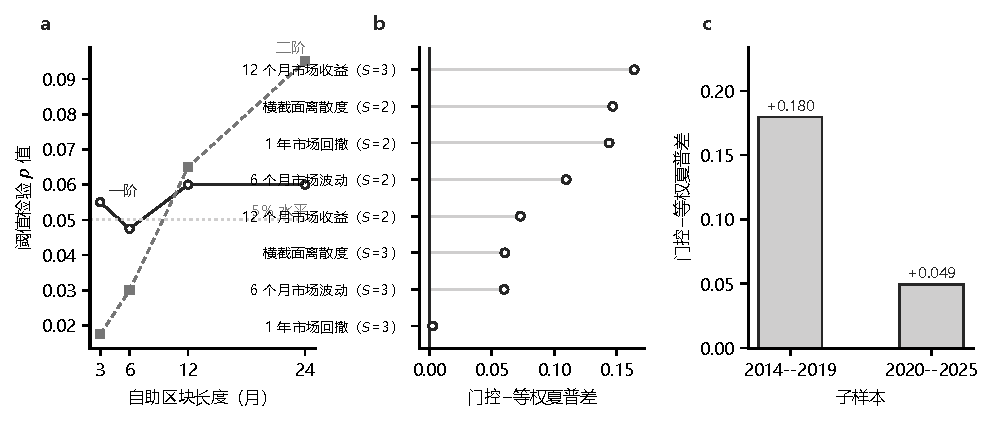
\includegraphics[width=\textwidth]{fig_robustness.pdf}
\caption{稳健性检验汇总}
\label{fig:robustness}
\begin{minipage}{0.94\textwidth}\footnotesize
注：(a) 阈值检验的 $p$ 值随自助区块长度变化，点线为 5\% 水平，一阶与二阶渠道
分别用实线圆点与虚线方点表示；(b) 四种制度变量与两种制度数下相对同期等权基准的
夏普差值；(c) 子样本的夏普差值均值，由主实验年度窗口汇总。
\end{minipage}
\end{figure}

十只美国 ETF 样本上的不可识别结果还有一层对照意义：该样本正是既有研究报告
「门控与等权不可区分」结论的样本。本文在该样本上重复得到相同结论，
并给出三重解释：绝对收益目标使门控退化（主动暴露 $0.0003$）；
横截面过窄使互补性统计量的上界低于噪声底线；样本期内制度持续性与互补性
都不足以支撑门控优势。既有实验的零结果在本文框架下对应三个具体预测的同时成立。
以少数资产为标的的多智能体研究与股票横截面研究之间，结论不宜互相外推。

本文结论受四项数据约束。样本覆盖方面，868 只证券来自公开行情接口在采集期内
仍可返回历史数据的证券集合，覆盖 A 股主板与创业板的主要部分，
不等于全部 A 股；退市缓冲仅覆盖 8 个可识别的真实退市观测，
退市损失因此被低估，结果相对乐观。考虑到核心结论是门控优势不显著，
该方向性偏差不改变主要判断。变量口径方面，公开行情接口不提供换手率，
本文以异常成交量替代，该口径保留了相对自身历史的异常交易活跃度，
与流通股本口径不完全等同，主要影响低换手专家的信号质量。
频率方面，$\Theta^{(1)}\propto1/T$，日频或周频数据可在相同时间跨度内提供更多观测，
本文结论不应外推为门控在日频上也无价值。信号集方面，五个专家信号全部基于价量特征，
引入估值、盈利质量或文本情绪信号可能提高专家分歧度，从而改变 $\hat\Gamma$ 的量级，
这是本文框架的直接可检验扩展。制度状态的划分在本文中为外生分位划分，
改用马尔可夫状态切换模型内生估计状态会引入额外估计误差（提高 $\Theta$），
同时可能提高制度划分的准确性，两者净效应需另行检验。

\begin{table}[htbp]
\centering
\caption{理论预测与实证结果对照}
\label{tab:verdict}
\begin{threeparttable}
\footnotesize
\begin{tabular}{lp{4.2cm}p{4.6cm}l}
\toprule
编号 & 理论预测 & 实证结果 & 判定 \\
\midrule
H0 & $\hat\Gamma>\Theta$ 时门控占优 & 未越过阈值，$p=0.060$ / $0.065$ & 未支持（临界） \\
H1 & 制度数内点最优 & $S=3$ 处最高，$3\to4$ 转为下降 & 支持（方向） \\
H2 & 宽横截面才可识别；二阶渠道更易识别 & 窄样本不可识别；二阶 $p=0.065$ & 支持 \\
H3 & 成本上升降低门控优势 & 每 10 基点 $-0.0147$，$p<0.001$ & 支持 \\
H4 & 样本越长越易占优 & 斜率 $-0.006\,3$，$p=0.617$，非单调 & 不支持 \\
H5 & 持续性放大互补性价值 & $\Corr=0.985$，放大 19.5 倍 & 支持（方向） \\
H6 & 无互补性则门控收益为零 & 安慰剂使主动收益归零 & 支持 \\
H7 & 绝对收益目标导致退化 & 主动暴露降至 $0.03\%$ & 支持 \\
\bottomrule
\end{tabular}
\begin{tablenotes}[flushleft]\footnotesize
\item 注：H0--H7 的定义见表 \ref{tab:theory-map}。
「未支持（临界）」指统计量未越过 5\% 水平的噪声底线但逼近该底线，
与门控组合经济量级明显、统计不显著的表现一致。
\end{tablenotes}
\end{threeparttable}
\end{table}

表 \ref{tab:verdict} 汇总全部检验：八个可检验含义中五个得到支持（其中三个为方向性支持），
一个不支持，一个为临界结果，一个（H0）未能在 5\% 水平上通过。
大部分方向正确、关键阈值临界，这一组合模式构成本文最重要的实证结论：
多智能体门控运行在可识别性的边界上。
